\paragraph{QuizziPedia::Front-End::Views::QuestionnaireManagementView}
\begin{figure} [ht]
	\centering
	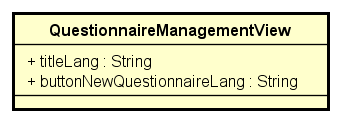
\includegraphics[scale=0.80]{UML/Classi/Front-End/QuizziPedia_Front-end_QuestionnaireManagementView.png}
	\caption{QuizziPedia::Front-End::Views:QuestionnaireManagementView}
\end{figure} \FloatBarrier
\begin{itemize}
	\item \textbf{Descrizione}: view principale per la gestione dei questionari;
	\item \textbf{Utilizzo}: permette di visualizzare tutti i questionari creati, quelli abilitati per la compilazione e quelli non ancora abilitati; contiene inoltre il link per la creazione di un nuovo questionario;
	\item \textbf{Relazioni con altre classi}:
	\begin{itemize}
		\item \textit{IN} \texttt{QuestionnaireManagementModelView}: classe di tipo modelview la cui istanziazione è contenuta all'interno della variabile di ambiente \$scope di \texttt{Angular.js}. All'interno di essa sono presenti le variabili e i metodi necessari per il \textit{Two-Way Data-Binding\ped{G}} tra la view \texttt{QuestionnaireManagementView} e il controller \texttt{QuestionnaireManagementController};
		\item \textit{IN} \texttt{EliminationAndModifyDirective}: direttiva contenente i componenti grafici  che permettono di eliminare un questionario o di modificarne uno esistente;
		\item \textit{IN} \texttt{ExamModalityDirective}: directive contenete i componenti grafici per attivare la modalità esame su un questionario e gestire le iscrizioni;
		\item \textit{IN} \texttt{QuestionnaireResultsDirective}: rappresenta il componente grafico che permette all'utente autenticato pro di vedere i risultati di chi ha compilato il questionario. Tale componente è contenuto nella lista dei questionari abilitati alla compilazione. \'E possibile accedere alla lista dei risultati azionando l'evento ad esso collegato;
		\item \textit{IN} \texttt{LangModel}: rappresenta il modello delle informazioni per la giusta traduzione dell'applicazione.
	\end{itemize}
		\item \textbf{Attributi}:
		\begin{itemize}
			\item \texttt{+ questionnaireList: Array} \\ Array contenente la lista dei questionari creati; ogni questionario sarà rappresentato come un oggetto;
			\item \texttt{+ titleLangQuestionnaireManagement: String} \\ Attributo che viene utilizzato per visualizzare la giusta traduzione del titolo della pagina, in italiano o in inglese;
			\item \texttt{+ buttonNewQuestionnaireLangQuestionnaireManagement: String} \\ Attributo che viene utilizzato per visualizzare la giusta traduzione della \textit{label\ped{G}} per il bottone di creazione di un nuovo questionario, in italiano o in inglese.
		\end{itemize}
\end{itemize}
